\section{Results} \label{sec:results}


\subsection{Setup}
We use a local setup of spark since we are interested in I/O speed and not in distribution.
Benchmarks are performed on an Intel i7-3820QM with 12GB RAM. The disk used was a HDD.

\subsection{Scenario I}
As described in Section \ref{sec:scenario-one}, this scenario does not feature nested objects.
We expect Parquet to massively outperform both JSON and CSV.
Intituitively, we also expect writing to Parquet being slower since it utilizes compression.

\subsubsection{Writing Data}
In Figure \ref{fig:write-one}, we show write time for one million rows and a varying number of columns.

\begin{figure}[h]
\caption{Writing Time for Scenario I}
\centering
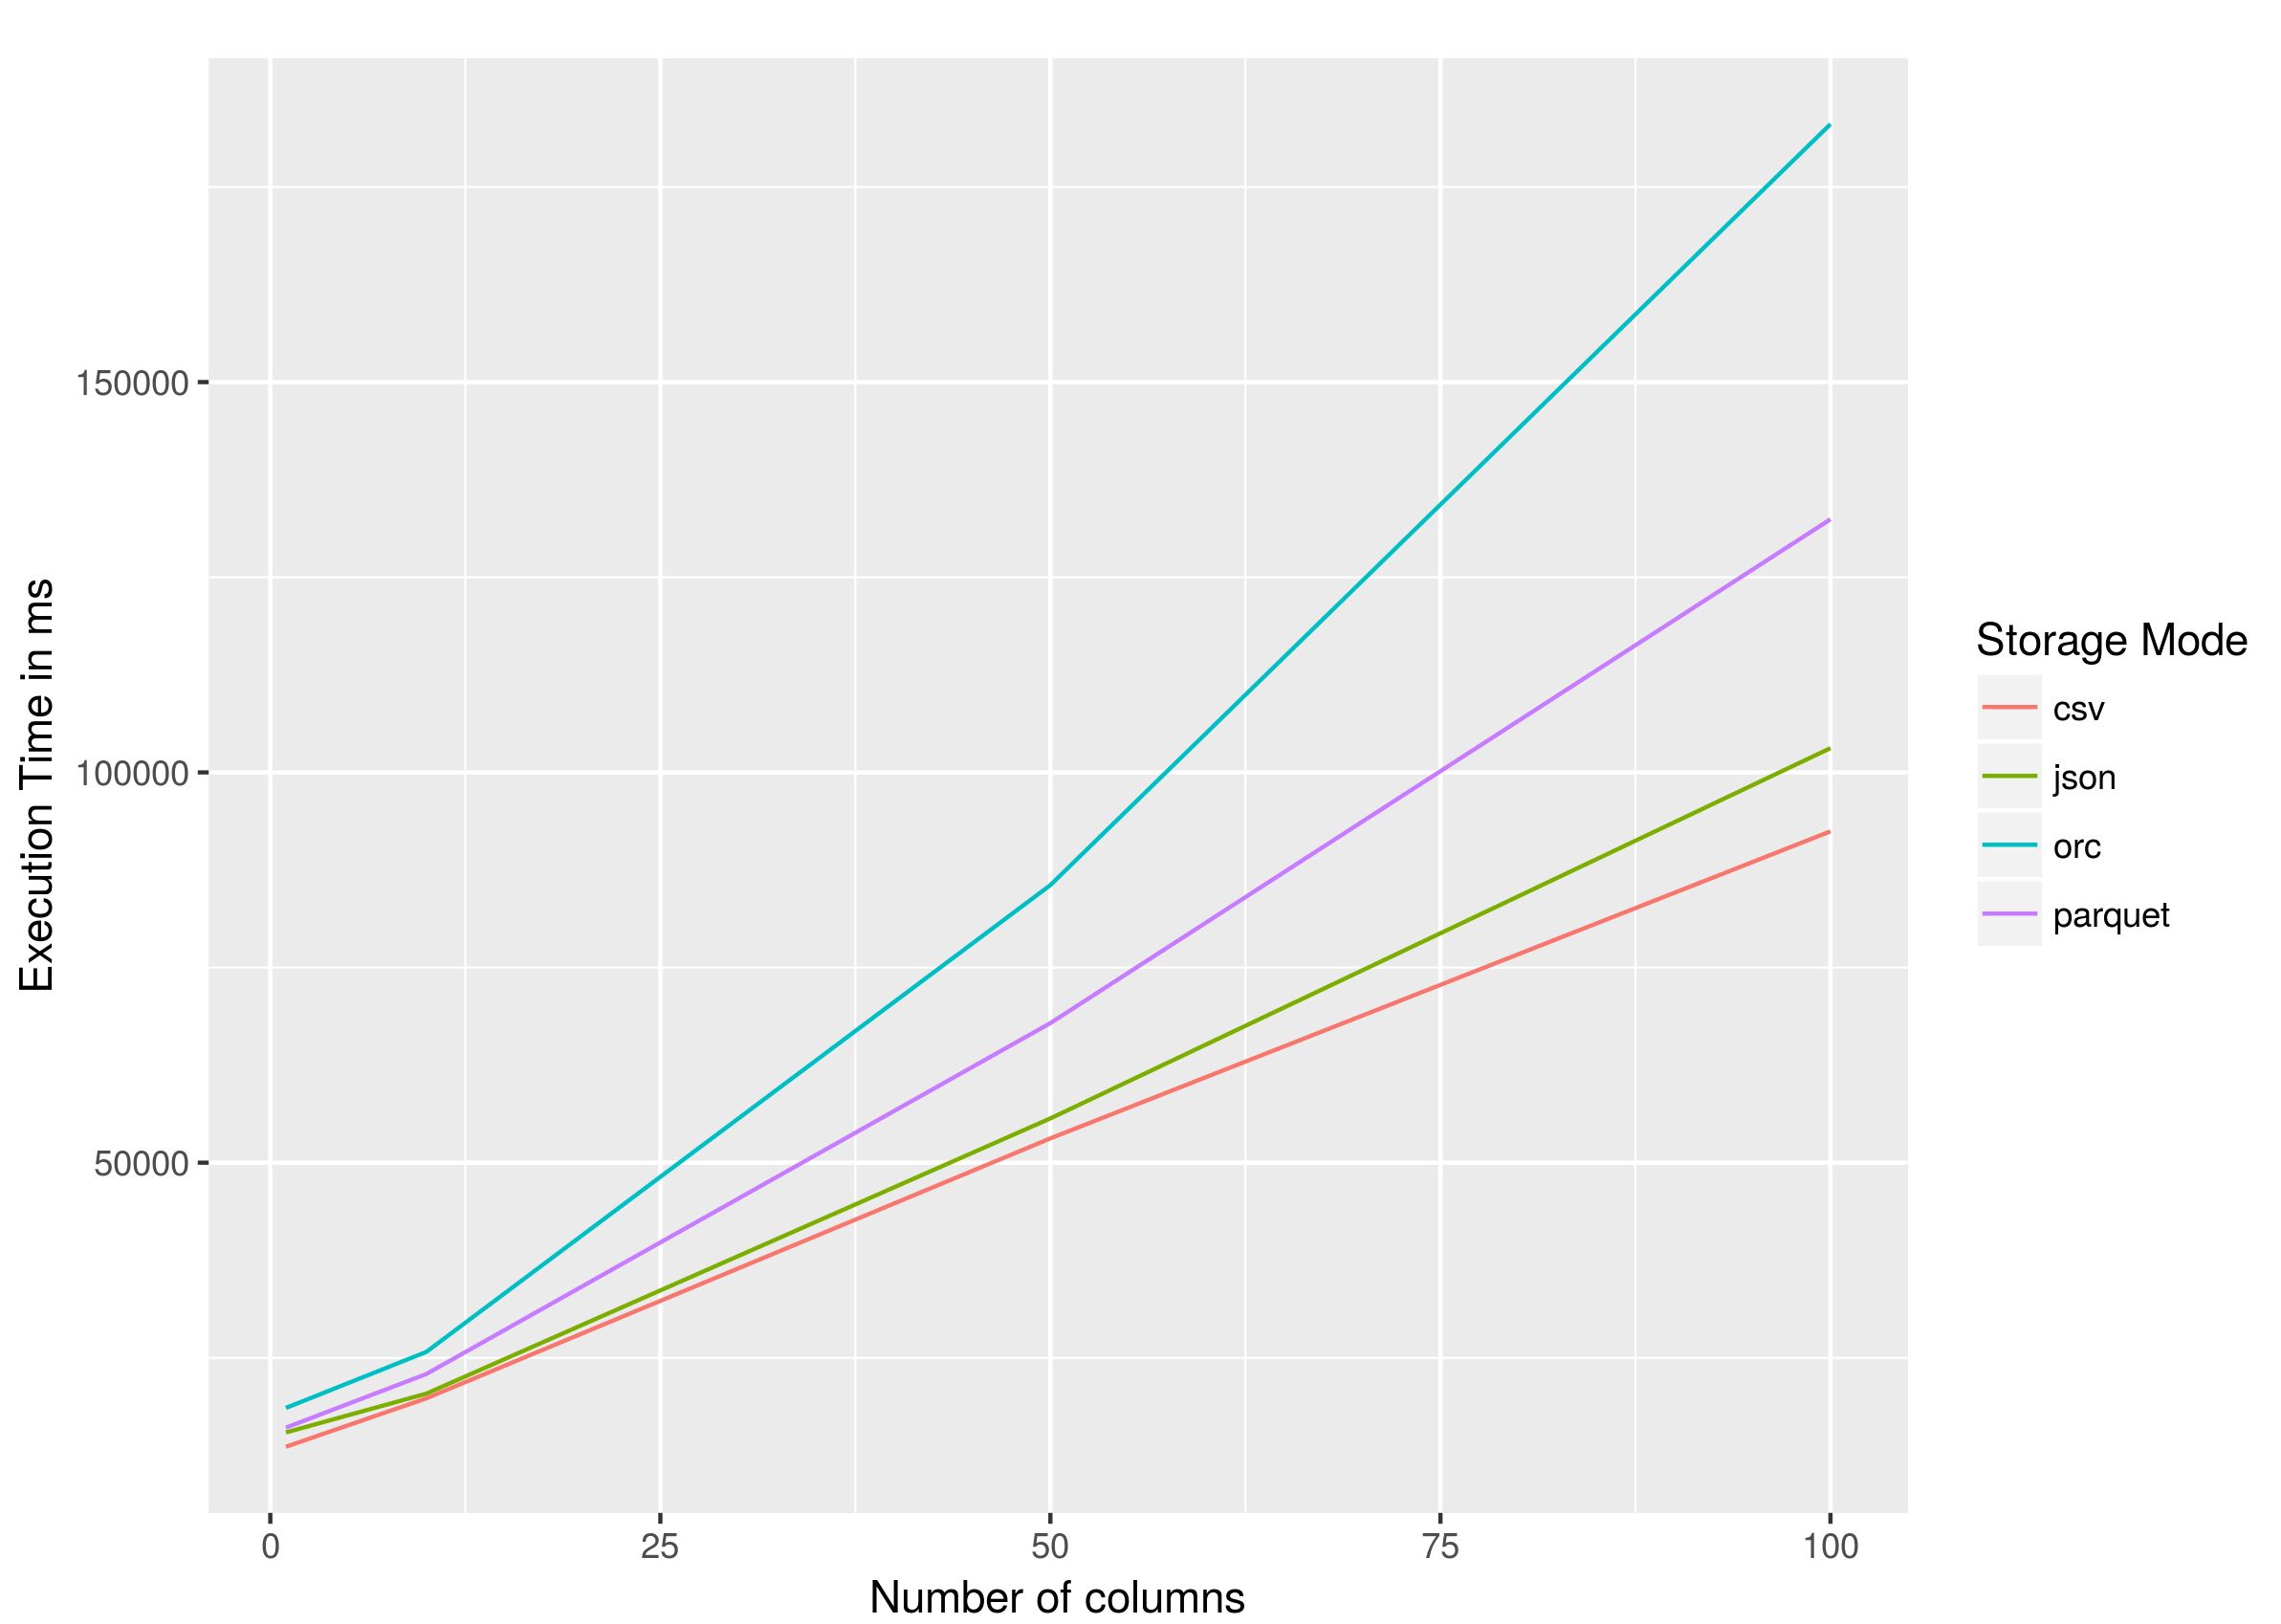
\includegraphics[width=1\textwidth]{write-one.png}
\label{fig:write-one}
\end{figure}

As expected, writing csv is fastest since json-files are larger. Parquet being slower is also expected.

\subsubsection{Query}
In Figure \ref{fig:query-one}, we show the execution time of the query described in Section \ref{sec:query-one} for one million rows and a varying number of columns.

\begin{figure}[h]
\caption{Query Execution Time for Scenario I}
\centering
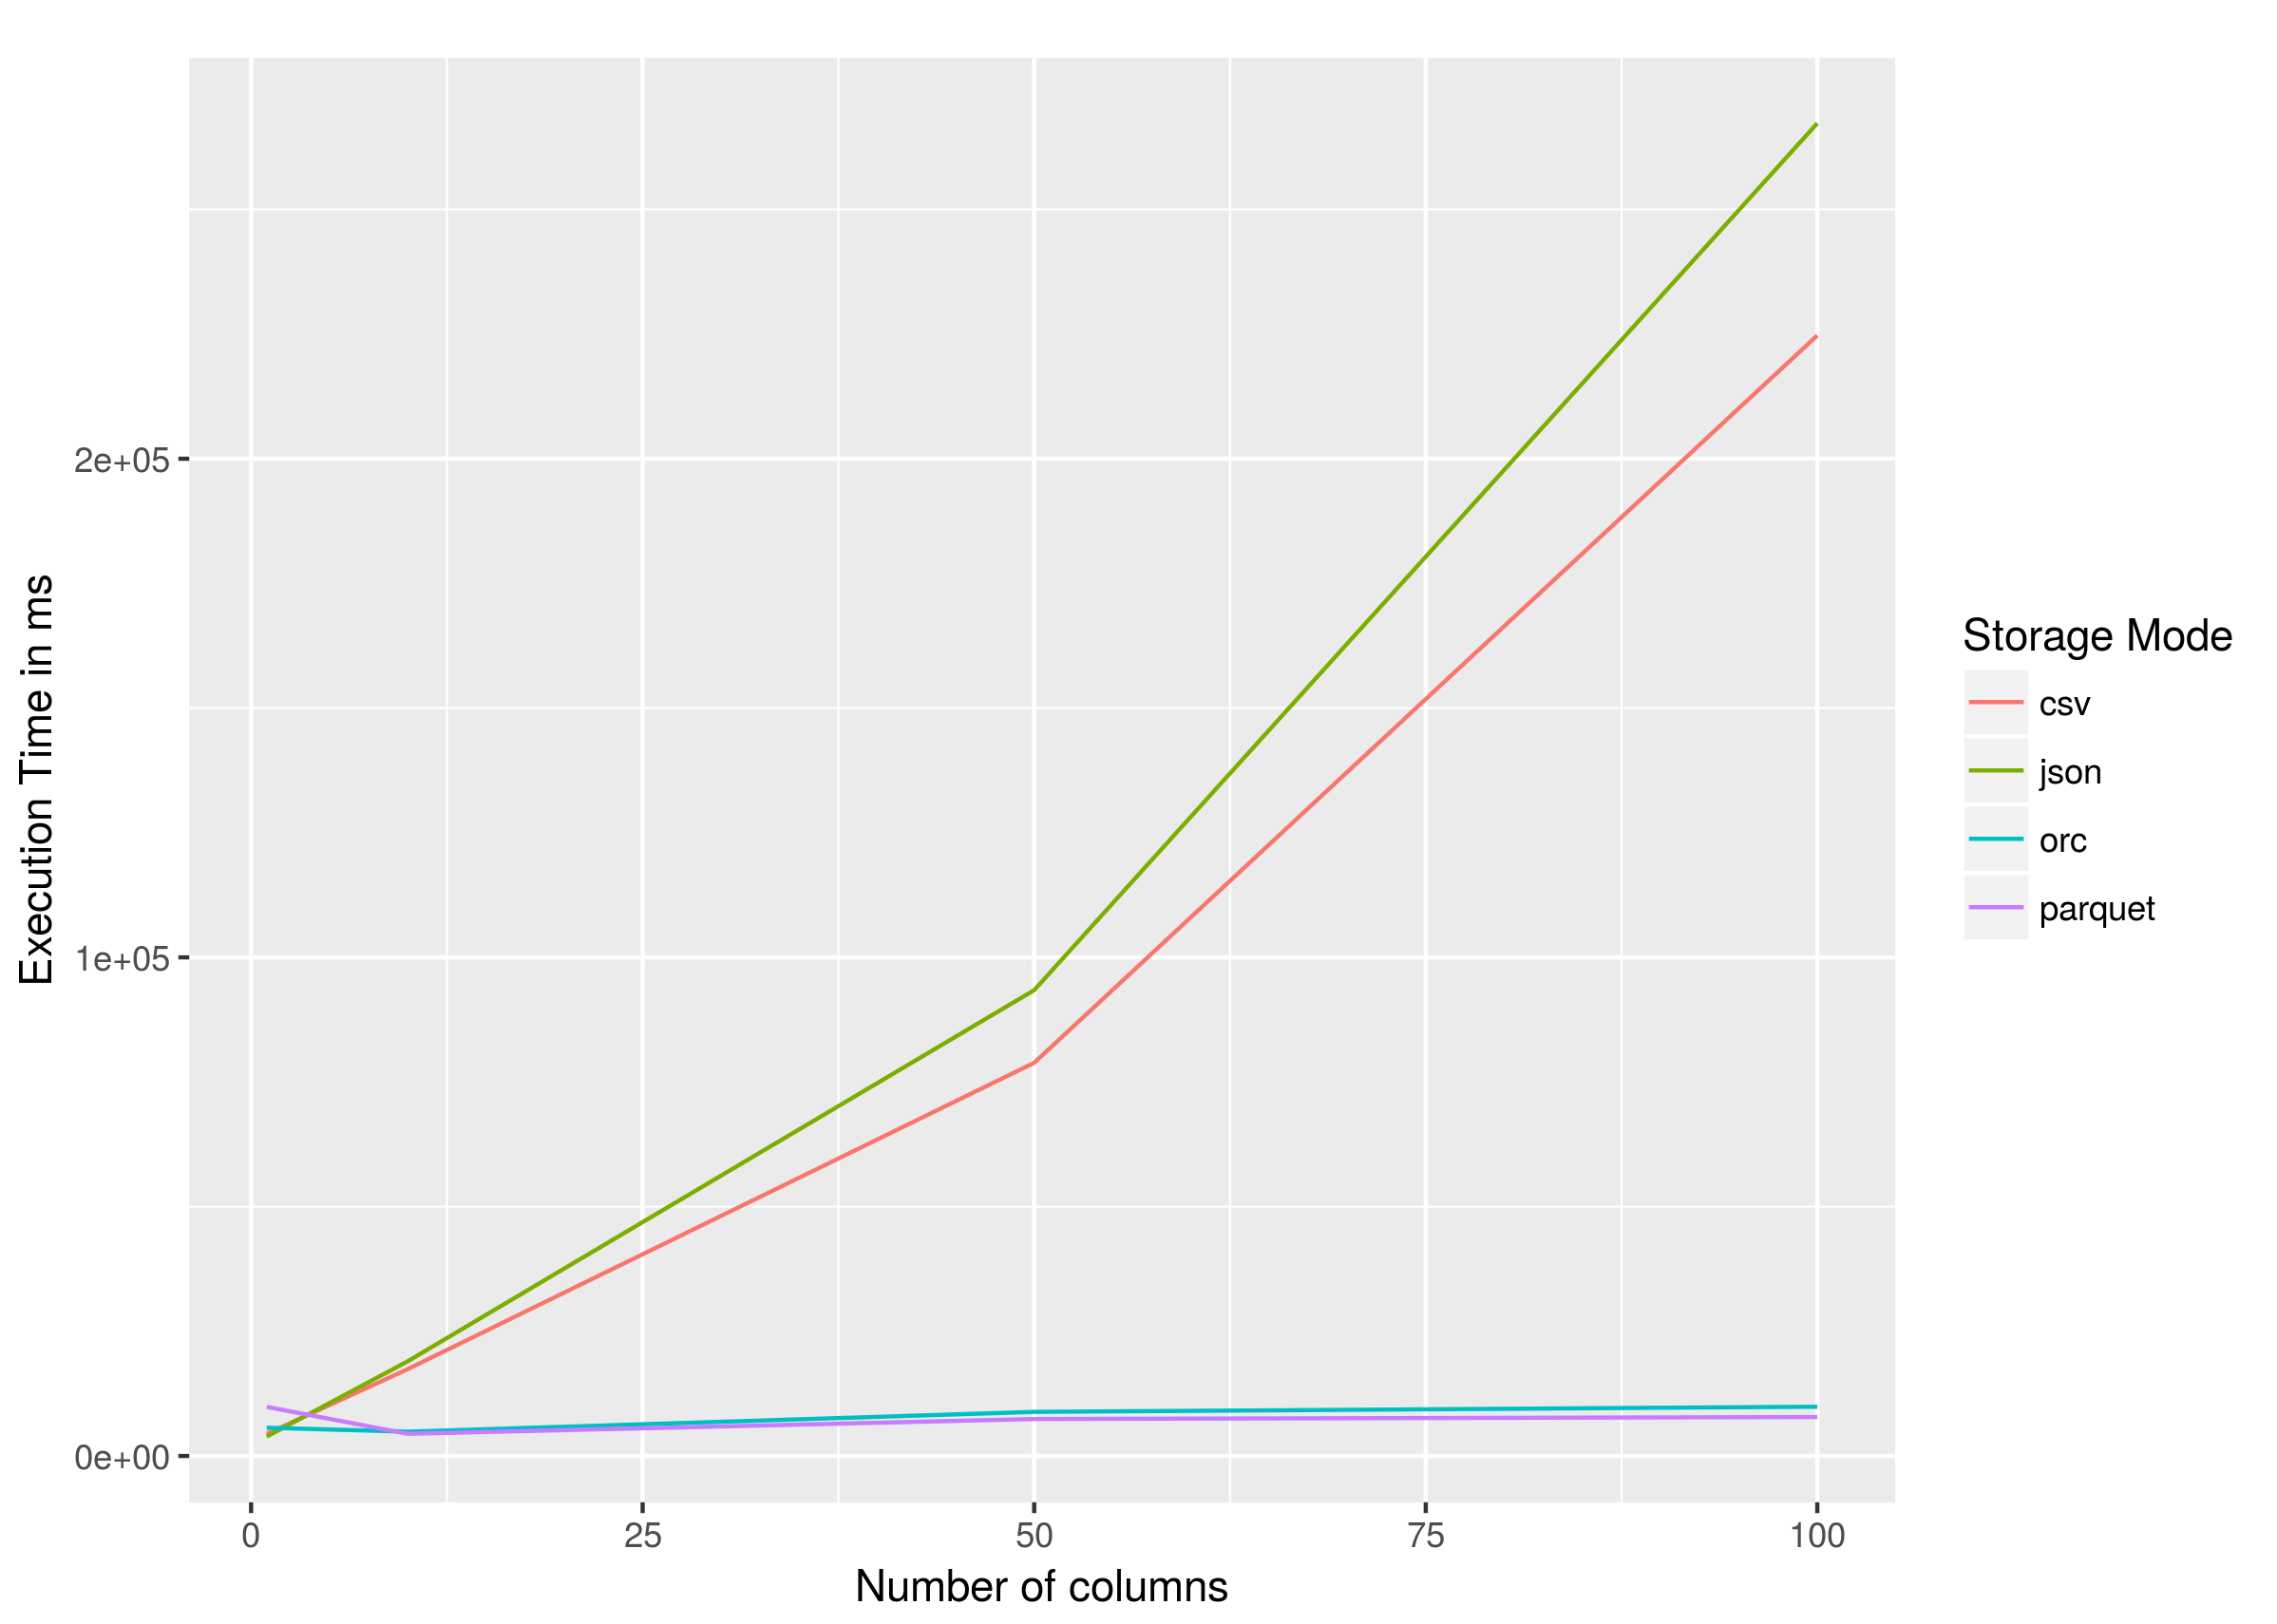
\includegraphics[width=1\textwidth]{query-one.png}
\label{fig:query-one}
\end{figure}

As expected, execution time for Parquet is constant as the number of column grows while execution time for JSON and CSV grows linearly.

\subsection{Scenario II}

